\documentclass{article}%
\usepackage[T1]{fontenc}%
\usepackage[utf8]{inputenc}%
\usepackage{lmodern}%
\usepackage{textcomp}%
\usepackage{lastpage}%
\usepackage[head=40pt,margin=0.5in,bottom=0.6in]{geometry}%
\usepackage{graphicx}%
%
\title{\textbf{Familiares de presos ultimados en Caricuao denunciarán ante Fiscalía militar}}%
\author{Diario El Universal}%
\date{02/12/2018}%
%
\begin{document}%
\normalsize%
\maketitle%
\textbf{URL: }%
http://www.eluniversal.com/sucesos/27241/familiares{-}de{-}presos{-}ultimados{-}en{-}caricuao{-}denunciaran{-}ante{-}fiscalia{-}militar\newline%
%
\textbf{Periodico: }%
EU, %
ID: %
27241, %
Seccion: %
sucesos\newline%
%
\textbf{Palabras Claves: }%
NO\_TIENE\newline%
%
\textbf{Derecho: }%
1.1%
, Otros Derechos: %
NO\_TIENE%
, Sub Derechos: %
1.1.1.6%
\newline%
%
\textbf{EP: }%
NO\newline%
\newline%
%
\textbf{\textit{Este ocurrió el miércoles pasado en el comando de la Guardia Nacional Bolivariana . En este procedimiento fueron ultimados cinco reclusos.}}%
\newline%
\newline%
%
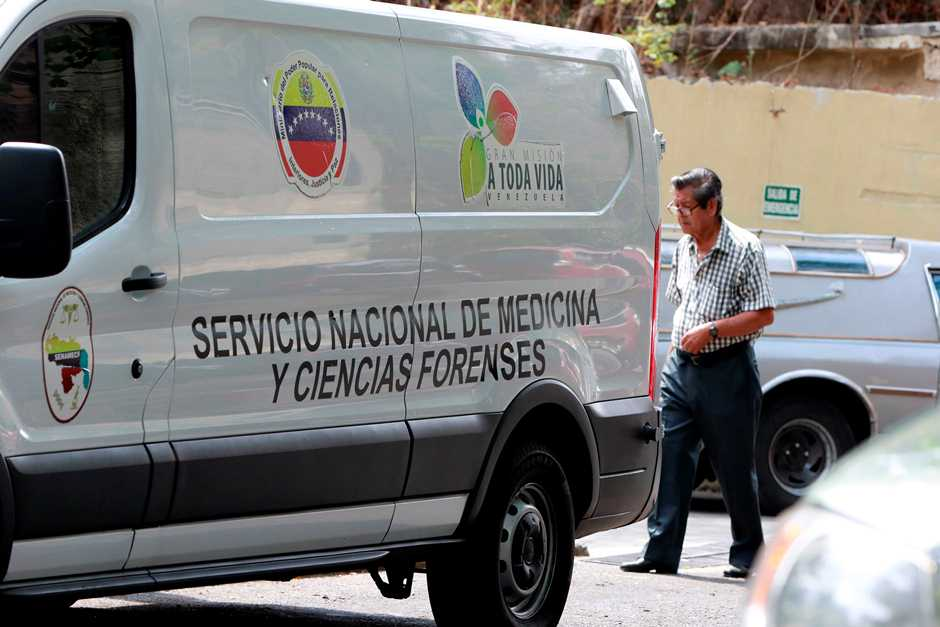
\includegraphics[width=300px]{86.jpg}%
\newline%
%
Familiares de los cinco presos que murieron durante el presunto intento de fuga del comando de la Guardia Nacional Bolivariana de Macarao, frente a La Gran Parada, se organizan para denunciar abuso y exceso de los funcionarios que actuaron en el procedimiento, así como maltratos y violaciones a los derechos humanos que sufrieron durante la reclusión, según reseña una nota del%
\newline%
%
Al amanecer del miércoles 28 de noviembre, se registró la presunta fuga en el comando militar, cuando procedían a realizar un traslado. Los familiares no han recibido ninguna versión oficial pero manejan distintas informaciones extraoficiales sobre lo ocurrido. Les dijeron que los presos fueron baleados dentro del mismo destacamento, también que les dieron “ley de fuga”, es decir, les permitieron correr y luego les dispararon. Otra versión señala que salieron por la puerta principal, ya que estaban presos en las escaleras.%
\newline%
%
Los parientes se encontraban a finales de semana en los funerales, pero anunciaron que a partir del lunes planificarán acudirán al Fuerte Tiuna, para pedir una investigación ante un fiscal militar, respecto al comportamiento de los efectivos castrenses.%
\newline%
%
Entre los fallecidos se encontraban Jean Carlos Sánchez Bandrés, escolta, de 37 años, Jorge Eliécer Castaño Fuentes (30), comerciante informal, y Nelson Antonio Adharsingh Velásquez (34).%
\newline%
%
Se supo que el cuarto fallecido era un joven de 20 años, que fue retirado de la morgue la tarde del viernes, y el quinto cayó abatido en un hecho aislado.\newline%
\newline%
Los familiares denunciaron que los cuerpos presentaban más de un disparo y golpes.%
\newline%
%
El protocolo de autopsia de Sánchez Bandres indica que murió por proyectil único, de arma de fuego, en el costado izquierdo con salida por el estómago, que le causó shock hipovolémico, pero cuando vestían el cadáver en la funeraria se percataron que tenía dos tiros más, a quemarropa, en la espalda, golpes en brazos, piernas, barbilla, nariz y hombro derecho.%
\newline%
%
Durante la reclusión, los presos recibían visita de un familiar durante cinco minutos. Los guardias revisaban la comida con las manos y les sacaban la carne ó el pollo, para dejarles solo los contornos (arroz o pasta).%
\newline%
%
\end{document}